% !TEX root = ../proj_report_outline.tex

\chapter{Proposed Architectures}\label{C:arch}
In this chapter we use the intuitions gathered from related works to propose novel classes of
architectures employing tensor decompositions to implement multiplicative connections. We term this
family of architectures \emph{Recurrent Tensor Networks} to emphasise their explicit incorporation
of a decomposed tensor. There are
two key principles: simplicity and modularity. We want to design networks that have no extraneous
components so that every element of the network has a clearly defined role. We first propose
two novel architectures utilising a tensor product and then explain the decisions that led to their
construction.

\section{Architectures}
\subsection{Biases}
Neural networks typically require biases to be able to express a full range of transformations. We would
expect a tensor layer to be no different. A common way to conceptualise the addition of a bias for a
given layer is to incorporate it into the weight matrix by adding an additional row and inserting a
corresponding input which has its value fixed to one. 
We use \(\tilde{\phantom{x}}\) to represent altering the inputs
and weights in this way: \(\tilde{\vec{x}}\) is an input vector with an additional \(1\) appended
and \(\tilde{\mat{U}}\) is a matrix with a corresponding additional row.

Generalising this construction to a three-way tensor we have to take an \(n_1 \times n_2 \times n_3\)
tensor to size \(n_1 + 1 \times n_2 \times n_3 +1\). If we then perform a bilinear product and separate
back out the extra components, we find that as well as the expected bias vector we have
two bias matrices, one per input. For a three-way tensor \(\tensor{W}\),
\begin{equation}\label{eq:tensorbias}
	\tran{\tilde{\vec{x}}}\widetilde{\tensor{W}}\tilde{\vec{y}}
	= \tran{\vec{x}}\tensor{W}\vec{y} + \mat{U}\vec{y} + \mat{V}\vec{x} + \vec{b}.
\end{equation} This is very similar to the manner in which the states are computed in the vanilla
RNN with the addition of the multiplicative tensor interactions.

Applying the same process when the tensor is represented in the CP decomposition does not
have the same result. Instead it results in adding bias vectors to two of the internal
matrix products. Let \(\tensor{W} = [A, B, C]_{CP}\), then appending ones to the inputs
results in
\begin{equation}
	\tran{\tilde{\vec{x}}}\widetilde{\tensor{W}}\tilde{\vec{y}}
	= \tran{\mat{B}}\left( (\mat{A}\vec{x} + \vec{b}_x) \odot (\mat{C}\vec{y} + \vec{b}_y)\right).
\end{equation} This is quite different to eq.~\eqref{eq:tensorbias}. If we wish to
insert such a tensor product into a neural network we must choose whether to leave the biases in
the decomposition or treat the bias matrices separately. The latter provides less control over the
parameters, as there are now two matrices unaffected by the rank, but it might be helpful in that we
could use a very low rank decomposition and still maintain a baseline behaviour. Further, separating
the matrices ensures the tensor product can at least behave in the same manner as a Vanilla RNN block.

\subsection{Generalised Multiplicative RNN}\label{sec:gmrnn}
The simplest architecture way to incorporate a decomposed tensor is to use it to generalise the
Multiplicative RNN, Multiplicative Integration RNN \autocite{Martens2011a, Wu2016} and Vanilla RNN.
To do this, we simply replace the various linear operations with a bilinear form with appropriate
biases:
\begin{equation}\label{eq:gmrnn}
	\vec{h}_t = \tau\left( \tran{\tilde{\vec{x}}_t}\tilde{\tensor{W}}\tilde{\vec{h}}_{t-1} \right)
\end{equation}
Choosing to keep the biases elements separate from the decomposition gives a form which captures
vanilla RNNs as well as several types of multiplicative RNNs:
\begin{equation}\label{eq:gmrnnbias}
	\vec{h}_t = \tau\left(\tran{\vec{x}_t}\tensor{W}\vec{h}_{t-1}
		+ \mat{U}\vec{h}_{t-1} + \mat{V}\vec{x}_t + \vec{b}\right).
\end{equation} We term this the Generalised Multiplicative RNN (GMR). Unfortunately this
network will still exhibit the same vanishing gradients as the vanilla RNN as the state updates
still pass through a matrix (albeit one modulated by the new input).

\subsection{Tensor Gate Unit}
Incorporating ideas from gated RNNs such as the LSTM and GRU, we also propose the following architecture,
which we call the Tensor Gate Unit (TGU):
\begin{align}\label{eq:tgu}
	\vec{h}_t &= \vec{p}_t \odot \vec{h}_{t-1} + (\vec{1}-\vec{p}_t)\vec{z}_t \\
	\vec{p}_t &= \sigma\left(\tran{\tilde{\vec{x}}}_t\widetilde{\tensor{W}}\tilde{\vec{h}}_{t-1} \right)\\
	\vec{z}_t &= f(\mat{W}_{in}\vec{x}_t + \vec{b}_{in})
\end{align}
Where \(f(\cdot)\) is either a linear rectifier or the identity function.

\section{Motivation}
The GMR is an elegant generalisation of a number of fairly simple architectures. However, it will
still suffer from vanishing gradients and correspondingly we do not expect it to be capable of
learning long time dependencies. To solve this in the TGU we incorporate several
key ideas from the LSTM and the GRU. This section explains in detail the decisions taken and
the analysis behind them.

\subsection{Solving Vanishing Gradients}\label{sec:additive}
The biggest issue with the GMR and Vanilla-style RNNs in general is vanishing gradients.
A simple approach to avoid this
 is to have the network compute a candidate state update
\(\vec{z}_t\) and obtain new hidden states as
\begin{equation}\label{eq:additiveupdate}
	\vec{h}_k = \vec{h}_{k-1} + \vec{z}_k.
\end{equation}

Recalling eq.~\eqref{eq:bptt-v}, the problematic term was \(\nabla_{\vec{h_{k-1}}}\vec{h}_k\),
the gradient of a hidden state with respect to its immediate precursor. If the state is computed by
eq.~\eqref{eq:additiveupdate}:
\begin{equation}\label{eq:additivegrad}
	\nabla_{\vec{h}_{k-1}}\vec{h}_k = \mat{I} + \nabla_{\vec{h}_{k-1}}\vec{z}_k.
\end{equation} Adding the identity matrix adds one to each eigenvalue of the gradient, which ensures
that at least.

While the gradients may not vanish, they are likely to explode. Pascanu et al. show that a necessary
condition for exploding gradients is that the largest
eigenvalue of this gradient is greater than one \autocite{Pascanu2012}. For this
additive update all we require for exploding gradients is then for
\(\nabla_{\vec{h}_{k-1}}\vec{z}_ k\) to have at least one positive eigenvalue. This is highly likely
 from random initialisation, so this architecture is going to be challenging to train.
Additive connections give us a way to fight vanishing gradients, but we need to temper them somehow
to avoid exploding gradients. Fortunately, LSTMs and GRUs already present a class of successful
techniques for this.
%There
%is also a more intuitive reason why this network is na\"ive: it
% will struggle to forget. At each step, it will always add to the current state. Therefore,
%the candidate state must contain negative values to ever remove any information from the state. This
%suggests two things: the candidate state must depend on the previous state (so that it knows what to
%remove) and that the network will need to be very precise so that it can
%actually remove information that is no longer necessary. This last point suggests 
% trouble if the non-linearity applied to the candidate states is bounded -- if it erroneously
%adds during training it will struggle to learn to subtract if it can not hope to subtract the correct amount.
%An unbounded non-linearity would
%exacerbate the gradient issues, which makes this sort of a network challenging to design.


\subsection{Gates}\label{sec:gate}
LSTMs and GRUs manage their additive connections by applying multiplicative gates. We will therefore
investigate the solutions they present, with a view to choosing the best. We refer to the LSTM's gate
as a \emph{forget} gate. This type performs best
 in the presence of other gates \autocite{Greff2016, Jozefowicz2015}, which is explained by our 
 theoretical analysis.
The gate on the GRU is slightly
different and has a number of advantageous properties which lead to its eventual selection.
We term this the \emph{convex} gate as it recursively computes convex sums. 

Both of these gates apply element-wise. Although as multiplicative structures we could generalise
them with a tensor product, the element-wise nature is essential for keeping the gradients intact.
Applying a gate will replace the identity matrix in eq.~\eqref{eq:additivegrad}
with some other matrix. If the gating is done element-wise, then the new matrix will remain diagonal,
meaning it will still act purely additively on the eigenvalues of the gradient. If we allow a tensor
product, then we could be adding any arbitrary matrix into the gradient, which will exactly re-introduce
the pathologies we seek to avoid.

Denote by \(p_t\) the gate signal at time \(t\) (which is a
function of both the input and the current state and bounded in \([0, 1]\)). We also use
\(h_t\) to refer to the hidden state at time \(t\) and \(z_t\) will
refer to the candidate update computed by the rest of the network. In general these
elements are vectors but in the following we assume scalars with no loss of generality as
the vector forms contain only element-wise operations.

We define the
forget gate's recurrence as
\begin{equation}
	h_t = p_th_{t-1} + z_t.
	\label{eq:forgetgate}
\end{equation} The forget gate allows the network to wholly replace the
state with a new value.

The convex gate makes the following modification:
\begin{equation}
	h_t = p_th_{t-1} + (1-p_t)z_t.
	\label{eq:cvexgate}
\end{equation} While a simple adjustment, one gate signal is now able
to control the acceptance or rejection of new information.

In order to analyse the behaviour of these gates, we observe that each state \(h_t\)
can be expanded as a weighted sum over all \(z_i\) for \(i \leq t\). We can think of
the states as being a sliding-window sum over candidates where the shape of the window is defined
recursively by the \(p_i\) values.\footnote{There is in fact no sliding window -- the sum is always
over all values. However, given the range of window shapes the gating mechanism is capable of producing
it is reasonable to think about it as something close to a one-dimensional convolution.}
With this view in mind, we note that we can think of the
gate signals \(p_i\) as providing an \emph{attention} mechanism which controls how the network
attends to the information from past time steps.

\subsubsection{Forget Gate}
The forget gate allows the network to completely replace a state.
For this to happen the gate signal needs to be zero. If we define the initial
state \(h_0 = z_0\) we can write the first few states explicitly:
\begin{align}
	h_1 &= p_1z_0 + z_1 \\
	h_2 &= p_2h_1 + z_2 \\
		&= p_2(p_1z_0 + z_1) + z_2 \\
		&= p_2p_1z_0 + p_2z_1 + z_2.
\end{align} In general,
\begin{equation}
	h_t = \sum_{i=1}^{t-1} \left(\prod_{j=i+1}^t p_j\right) \cdot z_i + z_t.
\end{equation} Each state is a weighted sum of the past candidates, with strictly
non-increasing weights as we go back in time.
The coefficient of each past candidate is the product over all gate signals back from the
current time -- as the gate signals are in \([0, 1]\) it will reduce very rapidly the further
back we go.
Figure~\ref{fig:lstmgates} shows some possible resulting coefficients going back up to 1000 steps.
This leads to a key conclusion about this form of gate.

\begin{figure}[t]
\centering
\begin{subfigure}[t]{0.45\textwidth}
	\centering
	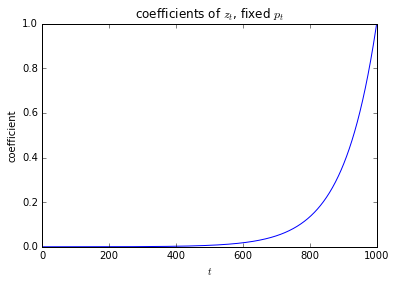
\includegraphics[width=\textwidth]{newarchs/lstmexp}
	\caption{Coefficients of \(z_t\) resulting from a fixed, high value of all \(p_t\)
	under the forget gate scheme.}
\end{subfigure}\hfill
\begin{subfigure}[t]{0.45\textwidth}
	\centering
	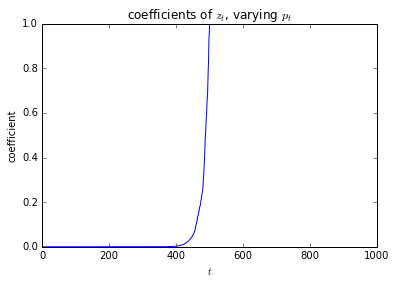
\includegraphics[width=\textwidth]{newarchs/lstmrect}
	\caption{Coefficients of \(z_t\) random \(p_t\) up to \(t=500\) and all \(p_t\) after
	500 set to 1.}
\end{subfigure}
\caption[Forget gate window shapes]
{Different window shapes produced by the forget gate. As each coefficient at time \(t\)
is the product of all gate values from \(t\) down to 1, the range of possible shapes is limited.}
\label{fig:lstmgates}
\end{figure}


\paragraph{Remembering requires cooperation.}
Consider the case where the network needs to remember an input at one time step and ignore all future
inputs. Achieving this with the forget gate can be done in two
ways. Firstly, the gate values can be clamped to one and the
candidates to zero. Clamping the gates to one produces an almost rectangular window; the state will be an
evenly weighted sum of all candidates from the point the gate switches on. All subsequent candidates
therefore must be zero.
A second method of remembering a single candidate state is by reproducing the same candidate
state at each time and setting the forget gate always to zero.

Both of these require a significant degree of co-operation between the gate and the mechanism that
produces candidate activations. Further, the production of candidate activations has to
depend on the previous state. The LSTM achieves this with additional gates controlling the candidate
production (which correspond to using a very unusual non-linear tensor decomposition). 
We hypothesise that this hinders learning as these components have to concurrently learn
complementary behaviours.

%\begin{figure}
%\centering
%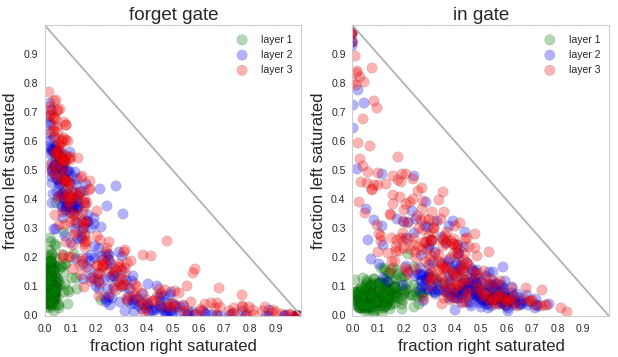
\includegraphics[width=0.6\textwidth]{newarchs/karpathy}
%\caption[Saturations of LSTM gates]{Saturation rates of 3-layer LSTM. The input gate modulates
%the candidate update, while the forget gate is as defined in this chapter. Figure from
%\autocite{Karpathy2016}, reproduced with permission.}
%\label{fig:karpathy}
%\end{figure}
%
%We hypothesise that the strong connection required between the candidate production
%mechanism and the forget gate indicates a strong potential for redundancy. Some experimental work 
%with LSTMs indicates that this may be the case.
%In \autocite{Karpathy2016} the authors trained a large LSTM on a language modelling task and
%plot the gates by the fraction of time they spend left-saturated (value \(<0.1\)) or 
%right-saturated (value \(>0.9\)). 
%This is reproduced in figure~\ref{fig:karpathy} and shows that the forget gates in general tend to spend
%more time in their lower ranges while input gates appear most likely to be in the higher ranges of their
%activation. This suggests most of the state is replaced at each time step (although
%looking at the input gate saturations, some cells must almost never change their value).

\paragraph{Gradients are gated.}
In order to update the weights of the network, we need the gradient of the hidden
state at each time \(t\) with respect to the gate signal at an earlier time \(i < t\):
\begin{align}
	\frac{\partial h_t}{\partial p_i} &= 
		\left(\prod_{k=i+1}^t \frac{\partial h_k}{\partial h_{k-1}}\right) 
			\frac{\partial h_i}{\partial p_i} = 
		\left(\prod_{k=i+1}^t p_k\right)
			h_{i-1} \\
\end{align} by eq.~\ref{eq:forgetgate}.
This makes it clear that the gating does not just happen during the forward pass. 
Repeating the process with respect to the candidate activations, it is clear that
the same argument applies.
\begin{align}
	\frac{\partial h_t}{\partial z_i} &= 
	\left(\prod_{k=i+1}^t \frac{\partial h_k}{\partial h_{k-1}}\right) 
	= \left(\prod_{k=i+1}^t p_k\right) \cdot
			1. \\
\end{align} If the gates
induce a strong decay, the network will be forced to update primarily on
local information and will struggle to learn long time dependencies.
A common practical solution is to initialise the bias of the unit computing the forget to a high
positive value so the gates start higher \autocite{Jozefowicz2015}.

\subsubsection{Convex Gate}
We now repeat the analysis with the convex gate. Let \(p_0 = 0\) and \(h_0 = z_0\) be some initial
state.
\begin{align}
	h_0 &= z_0 \\
    h_1 &= p_1z_0 + (1-p_1)z_1 \\
    h_2 &= p_2p_1z_0 + p_2(1-p_1)z_1 + (1-p_2)z_2 \\
%    h_3 &= p_3p_2p_1z_0 + p_3p_2(1-p_1)z_1 + p_3(1-p_2)z_2 + (1-p_3)z_3 \\
\end{align} giving rise to the general form
\begin{equation}
	h_t = \sum_{i=0}^t \left(\prod_{j=i+1}^t p_j\right) (1 - p_i) z_i
\end{equation} ensuring we define \(\prod_{j=i+1}^tp_j = 1\) if \(i = t\).
This is very close to what we had above, but the \(1-p_i\) term in the
coefficients has a significant impact. Firstly, we can prove the following statement which shows
that the sum over states is a convex sum.

\begin{prop} [Conservation of attention]
At any time \(t > 1\),
\begin{equation} \label{eq:cvexforward}
	\sum_{i=0}^t \left(\prod_{j=i+1}^t p_j\right) (1 - p_i) = 1.
\end{equation}
The coefficients of all previous candidates sum to one.
\label{prop:convexsum}
\end{prop}
\begin{proof}
If we expand the brackets, we can produce a telescoping sum. To ensure it telescopes
appropriately, we first pull the first and last terms out of the summation.
\begin{align}
    &\sum_{i=0}^t \left(\prod_{j=i+1}^t p_j\right) (1 - p_i) \\
    &= \prod_{j=1}^tp_j(1-p_0) + (1-p_t) + \sum_{i=1}^{t-1} \left(\prod_{k=i+1}^t p_k\right) (1 - p_i) \\
    &= \prod_{j=1}^tp_j(1-p_0) + (1-p_t) + \sum_{i=1}^{t-1} \left(\prod_{k=i+1}^t p_k\right) - \left(\prod_{l=i}^t p_l\right) \\
    &= \prod_{j=1}^tp_j(1-p_0) + (1-p_t) - \prod_{k=1}^t p_k + p_t \\
    &= \prod_{j=1}^tp_j - \prod_{k=1}^tp_k + 1 - p_0 + p_t - p_t = 1
\end{align}
\end{proof}
This means that the scale of the states
depends only on the scale of the candidate activations. Intuitively this should help address the danger
of exploding inherent in the additive update. We can make the following remarks about this form
of gate.

\begin{figure}[t]
\centering
\begin{subfigure}[t]{0.45\textwidth}
	\centering
	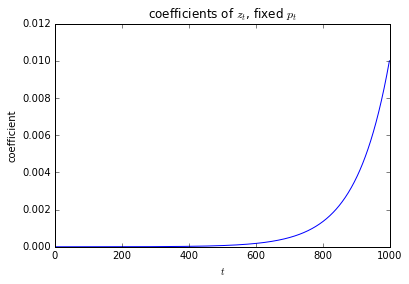
\includegraphics[width=\textwidth]{newarchs/cvexexp}
	\caption{Coefficients of \(z_t\) resulting from a fixed, high value of all \(p_t\)
	under the convex gate scheme.}
\end{subfigure}\hfill
\begin{subfigure}[t]{0.45\textwidth}
	\centering
	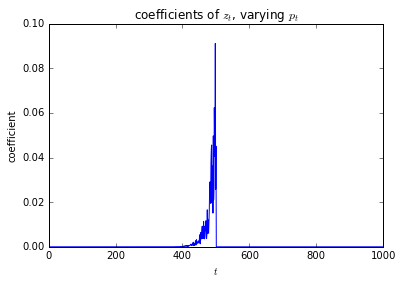
\includegraphics[width=\textwidth]{newarchs/cvexspike}
	\caption{Coefficients of \(z_t\) random \(p_t\) up to \(t=500\) and all \(p_t\) after
	500 set to 1.}
\end{subfigure}
\caption[Convex gate shapes]{Different window shapes produced by the convex gate.
 A simple adjustment to the formula allows
a much wider range of shapes.}
\label{fig:cvexgates}
\end{figure}

\begin{figure}[tbp]
\centering
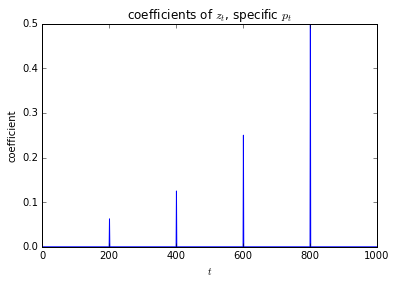
\includegraphics[width=0.45\textwidth]{newarchs/cvextrain}
\caption[Convex gate choosing several past candidates]
{Setting specific \(p_i\) to \(0.5\) picks out a set of past candidates, albeit with
an exponential decrease in their weighting.}
\label{fig:cvextrain}
\end{figure}

\paragraph{Remembering is easy.}
Figure~\ref{fig:cvexgates} illustrates two of the possible shapes this can take. It is clear
that this gating scheme provides a different set of possible shapes to work with.
Specifically, if the gate mechanism starts outputting values very close to one, the window
applied to past states takes the form of a distinct spike over a small range of activations.
This occurs because if \(p_i\) is very close to one, \(1 - p_i\) is very close to zero, so
state \(h_{i-1}\) is going to be carried over with only a very minor contribution from
\(z_i\). Figure~\ref{fig:cvextrain} further emphasises the difference, making it clear that
the convex gate is capable of representing a fundamentally different set of window shapes
than the forget gate, despite their similar formulation.

This enhanced range of window shapes makes these gates appealing as they may be able to reduce
interdependence between the gate mechanism and the candidate production mechanism. This may
allow us to remove the candidate's dependence on the previous state which should solve many of the
issues with the forget gate.

\paragraph{Gradients are still gated.}
The gradient of the hidden state \(h_t\) with respect to a previous gate signal
\(p_i\) has the form:
\begin{align}
	\frac{\partial h_t}{\partial p_i} &= 
		\left(\prod_{k=i+1}^t \frac{\partial h_k}{\partial h_{k-1}}\right) 
			\frac{\partial h_i}{\partial p_i} 
	= \left( \prod_{k=i+1}^t p_k \right) (h_{i-1} - z_i) \label{eq:cvexgrad}
\end{align}
While the gradient of the state with respect to a prior candidate is
\begin{align}
	\frac{\partial h_t}{\partial z_i} &=
		\left(\prod_{k=i+1}^t \frac{\partial h_k}{\partial h_{k-1}}\right) 
			\frac{\partial h_i}{\partial z_i}
	= \left( \prod_{k=i+1}^t p_k \right) (1 - p_i). \label{eq:cvexstategrad}
\end{align} The pattern here is fundamentally the same as the forget gate in that the gradient
is simply the coefficient assigned to \(z_i\) in the weighted sum that produced \(h_t\). Hence
all discussion of the differences in the gates' forward behaviour apply equally during the
backward pass.

Equation~\eqref{eq:cvexgrad} is interesting -- the gradient of the state with respect to the gate value
depends not just on the preceding state but on the difference between the state and the proposed
update. This means that during training what drives the updates is the possible changes that could be
made to the state, rather than just the state values itself. Meanwhile, eq.~\eqref{eq:cvexstategrad}
shows that proposition~\ref{prop:convexsum} also applies to the gradients. 
This suggests that as long as the scale of the candidate updates is under control
there will be no problems with exploding gradients.

The downside of the system is that it may still struggle to learn long time dependencies early.
It would be straightforward to initialise the gate so that it has a mean value of \(0.5\),
but this would correspond to an exponential decay of information. Unlike the forget gate simply
increasing the mean value (for example by initialising the bias to a high positive value)
will not correspond to a flatter window.


\subsubsection{Conclusions}
The convex gate by itself seems more capable than the forget gate as it is able to represent more
useful distributions over past candidate states where successfully employing a forget gate requires a more
complex method of producing candidate states. The convex gate avoids the issue of requiring
two components to learn complementary behaviours by allowing a single component to carry out the job.
This is appealing as it enables simpler and more modular architectures.


\subsection{Computing the gate}
In order to decide whether incoming information should
overwrite the current state values, the gate will need to see the current values and the new information.
The binary nature of this task suggests
the use of a tensor unit as discussed in chapter~\ref{C:tens}. Secondly if we want the full utility of
the convex gate, the mechanism to compute its values will have to be capable of modelling complex interactions. 
The bilinear tensor product is therefore
perfect fit.

It is also necessary to choose a non-linearity. We expect the gate to function mostly as a switch,
accepting or rejecting new information. The
typical approach is to ensure this smoothly with a sigmoid. Although sigmoids have undesirable
properties when used in feed-forward networks \autocite{Glorot2010} they remain the standard choice
when this kind of gating is desired \autocite{VandenOord2016, Oord2016} and we find no reason to
deviate from this, especially as keeping the gate activation bounded in \([0,1]\) will ensure the
gradients will not explode due to the additive connection.

Using a tensor in this fashion provides an interesting possibility: the ability to write to the memory
associatively. The gate is constantly computing weighted similarities between
the input and the current state so it is possible for the gate to react if a certain pattern in the
input matches a pattern stored in the state. This is a mode of behaviour very difficult to realise
with existing gated architectures \autocite{Danihelka2016}.

\subsection{Candidate update}
All that remains is to derive a candidate state update. Aside from Strongly Typed RNNs \autocite{Balduzzi2016}
and some Associative LSTM variants \autocite{Danihelka2016} this is usually performed via
a binary function of the current input and the previous hidden state. Intuitively this needs to
be the case with the standard LSTM style forget gate, but as we have decided against that it is worth questioning
the necessity of the previous hidden state in this calculation.

Removing this recurrent dependence makes each role in the network clearly defined. As each input arrives, it is
embedded into the state space. The gate then decides whether it is worth keeping.
The candidate production mechanism only needs to behave as a feature
detector, transforming the input into a representation that captures its essential structure.
Conceptually this is very clean and modular and therefore favourable provided it does not strip
the model of too much expressive power, which is best determined empirically.
%
%This scheme is appealing due to its simplicity and separation of
%roles, although two questions remain to be answered: how does this affect the expressive power of the
%network and how should we compute the necessary representation. The former is likely to be a best
%answered empirically, although we make a brief note here. A method for the GRU or LSTM to maintain
%information in their hidden states for long time periods is for the candidate production mechanism to
%learn an identity mapping from hidden states to hidden states. This behaviour is impossible to realise
%unless the candidate state depends on the previous hidden state. Note that this is also the only way
%that the Vanilla RNN can remember information for long time periods. Given the failures of the
%Vanilla RNN, we suggest that removing this mode of behaviour is no great loss. Further,
%we suggest it may help optimisation if there is only one clear way in which to store information.

What remains is to decide how to compute the candidate from the input. We wish to model a unary
mapping from the input to the candidate, so a logical way to proceed is with a standard feed-forward
layer:
\begin{equation}\label{eq:propcandidate}
	\vec{z}_t = f(\mat{W}_{in}\vec{x}_t + \vec{b}_{in}).
\end{equation} We experimented with a number of options for the non-linearity \(f\) and found the best
performance was consistently achieved with either a linear rectifier or no
non-linearity at all. This echoes trends in feed-forward networks away from saturating non-linearities
towards unbounded, piecewise linear activation functions \autocite{Goodfellow2013, He}. It is
interesting that for many tasks a linear candidate performed best -- clearly the
expressive power of the tensor combined with the non-linearity of to the gate is sufficient to
maintain the representative power of the network as a whole.

While a single feed-forward layer was sufficient in our experiments, there is scope to expand this
depending on the complexity of the task. For example this could be a deeper feed-forward architecture,
a convolutional neural network or even an identity map if the
input to the network is already high-level features.

